\section{Experimental Results}\label{sec:experimental-results}

We evaluate the PPO implementation of our auction framework on evolving reachability objectives and a heterogeneous extension combining feeding priorities and battery charging.
We compare against centralized PPO and DWN, and ablate observations, pooling, and auction hyperparameters.
A detailed description of the environments and the baseline approaches is provided in Appendix~\ref{app:experimental setup}, below we include a summary.
The supplementary material includes our codebase and recorded rollouts of our bidding-based policies on the three base environments.

\textbf{Environments.}
We evaluate our approach on three environments: a mobile cat feeder environment, introduced in Section~\ref{sec:introduction}, and the two Atari games Assault and Air-raid.
In all these environments, the metric being optimized is the cumulative reward across all objectives.

In the Cat Feeder environment, a robot moves on a $30\times 30$ grid to feed up to $m$ cats that move stochastically.
Each cat disappears after a fixed number of steps; feeding it yields a reward, while disappearance incurs a penalty of equal magnitude.
We train with $m=8$ cats in the environment and demonstrate generalization up to $14$.
Each cat is served by a dedicated policy whose observation includes the robot position, the locations of active cats, and their remaining lifetimes.
We ablate global observations with attention pooling, global observations with fixed concatenation (no pooling), and local observations only (blind).

In both the Atari games---Assault (Figure~\ref{fig:assault_preview}) and Air-raid---the agent controls a missile launcher to destroy incoming alien ships while avoiding enemy missiles~\citep{bellemare13arcade}.
Although this is not traditionally seen as a multi-objective environment, we treat each ship as a separate objective and assign a local policy to pursue it, enabling a modular and interpretable design.
In lieu of the standard pixel observations, we employ the object-centric variant of the Atari environments~\citep{delfosse2023ocatari} which provides the environment state information to the policies.
Destroying a target yields reward, losing a life incurs a penalty.
We do not use attention pooling in the Atari games since there are only up to 3 targets.


\textbf{Baseline approaches.}
We compare against two baselines: a single PPO policy optimizing the objective-aggregated reward and deep W-learning (DWN)~\citep{rosero2024multi}.
These baselines also access the same object-centric observations in the Atari games.
The PPO baseline is implemented using CleanRL~\citep{huang2022cleanrl}.
Since we provide distance-based reward shaping to help our policies learn, to ensure a fair comparison, we test nearest-target and earliest-expiry distance shaping, as well as urgency-weighted scalarization of objective rewards, in Cat Feeder.
Hyperparameters are provided in~\Cref{sec:reprod-details}.
PPO parameters for Cat Feeder were tuned using 40 Optuna iterations~\citep{akiba2019optuna} while standard CleanRL Atari hyperparameters were used for the Atari games.
The centralized PPO baseline is trained with the same number of environment samples as our method.
DWN trains one DQN policy per objective together with W-networks that estimate urgency scores of states.
We use the same action window \(\tau\) for DWN.
Training budgets are fixed in advance: 400 PPO iterations for Cat Feeder and Air-Raid, and 150 for Assault.
For each of ten runs, one seed initializes the environment and algorithm; evaluation uses subsequent non-overlapping draws from that seeded stream, rather than independently chosen seed identifiers.


\begin{figure}%[h]
    \centering
    \begin{subfigure}{0.32\textwidth}
        \centering
        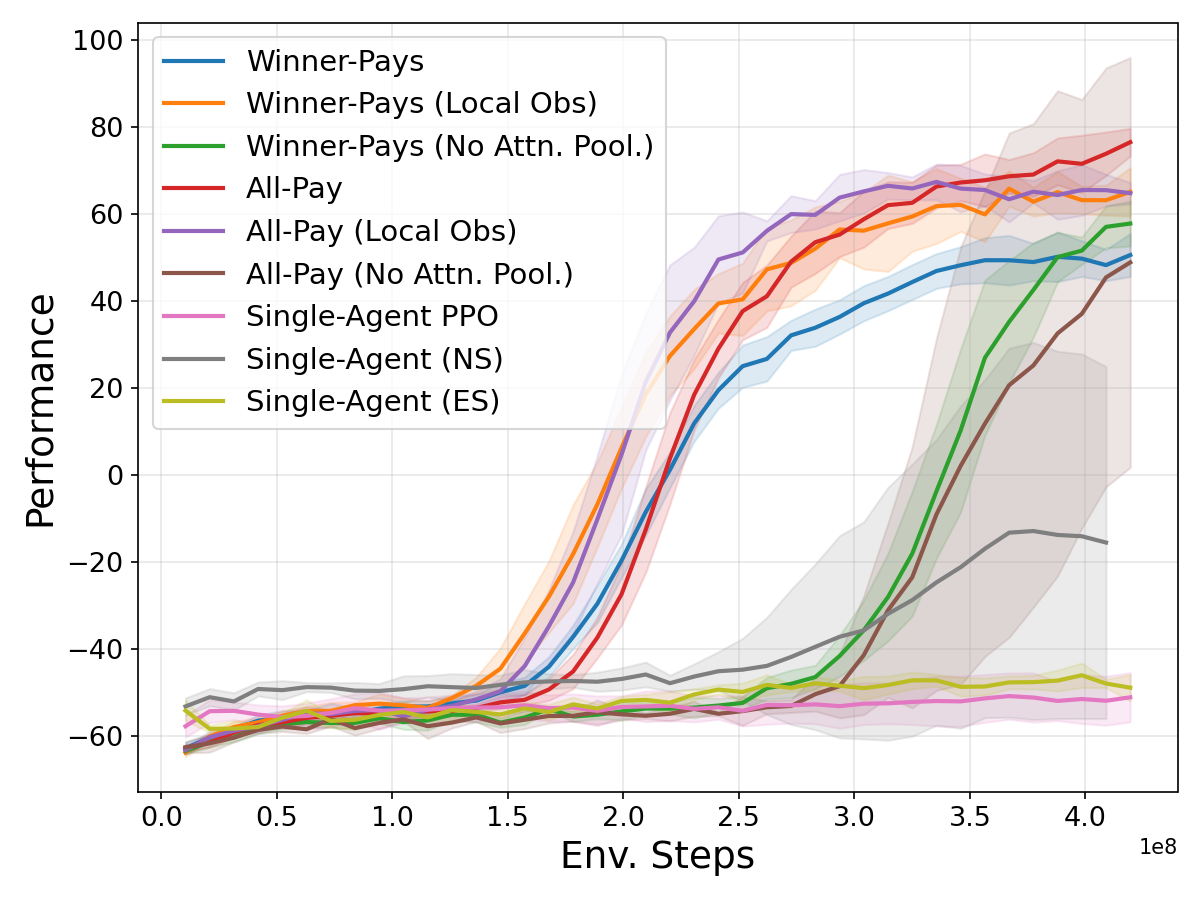
\includegraphics[width=\textwidth]{img/gridworld_bidding_mechanisms_learning_curves.png}
        % \caption{Cat Feeder: Learning curves}
        % \label{fig:dyntar-learning-curves}
    \end{subfigure}
    \hfill
    \begin{subfigure}{0.32\textwidth}
        \centering
        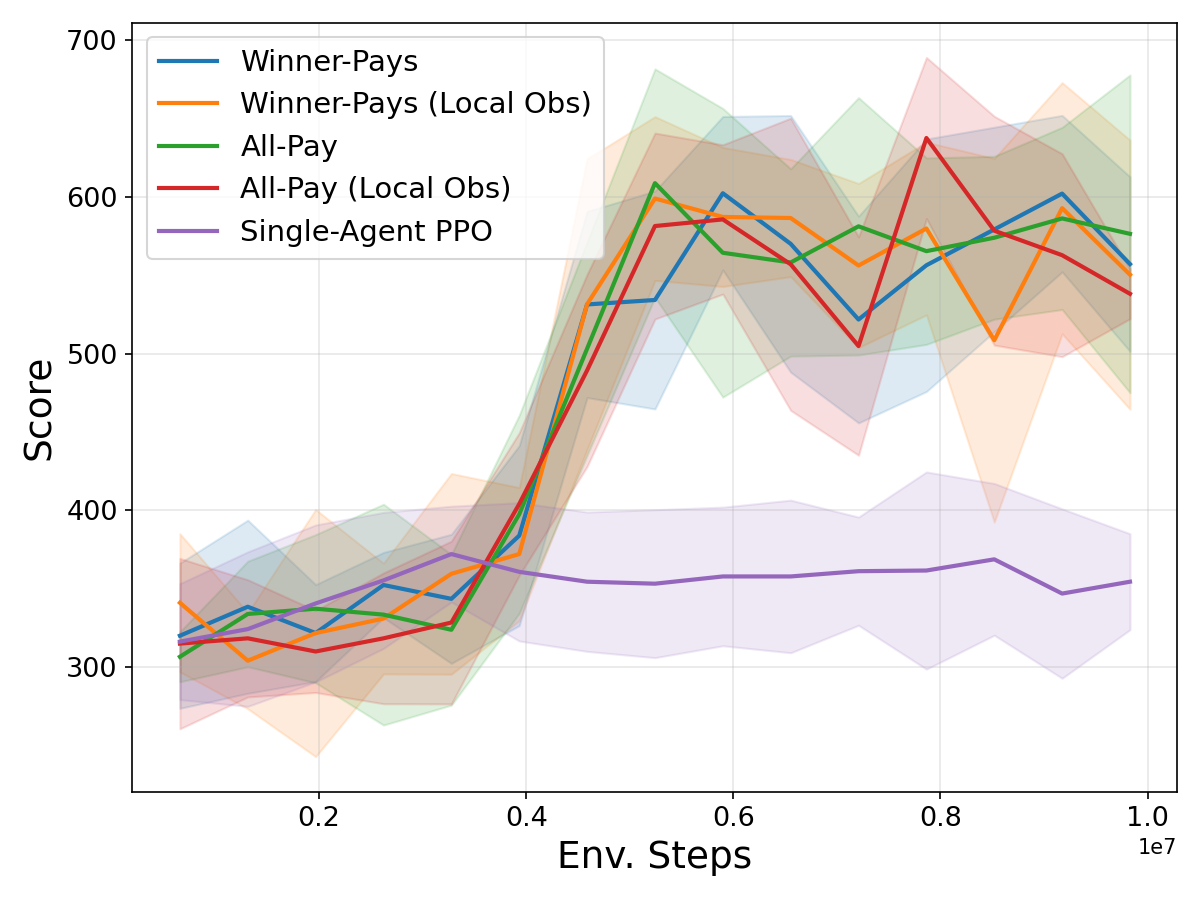
\includegraphics[width=\textwidth]{img/assault_bidding_mechanisms_learning_curves.png}
        % \caption{Atari Assault: Learning curves}
        % \label{fig:assault-learning-curves}
    \end{subfigure}
    \hfill
    \begin{subfigure}{0.32\textwidth}
        \centering
        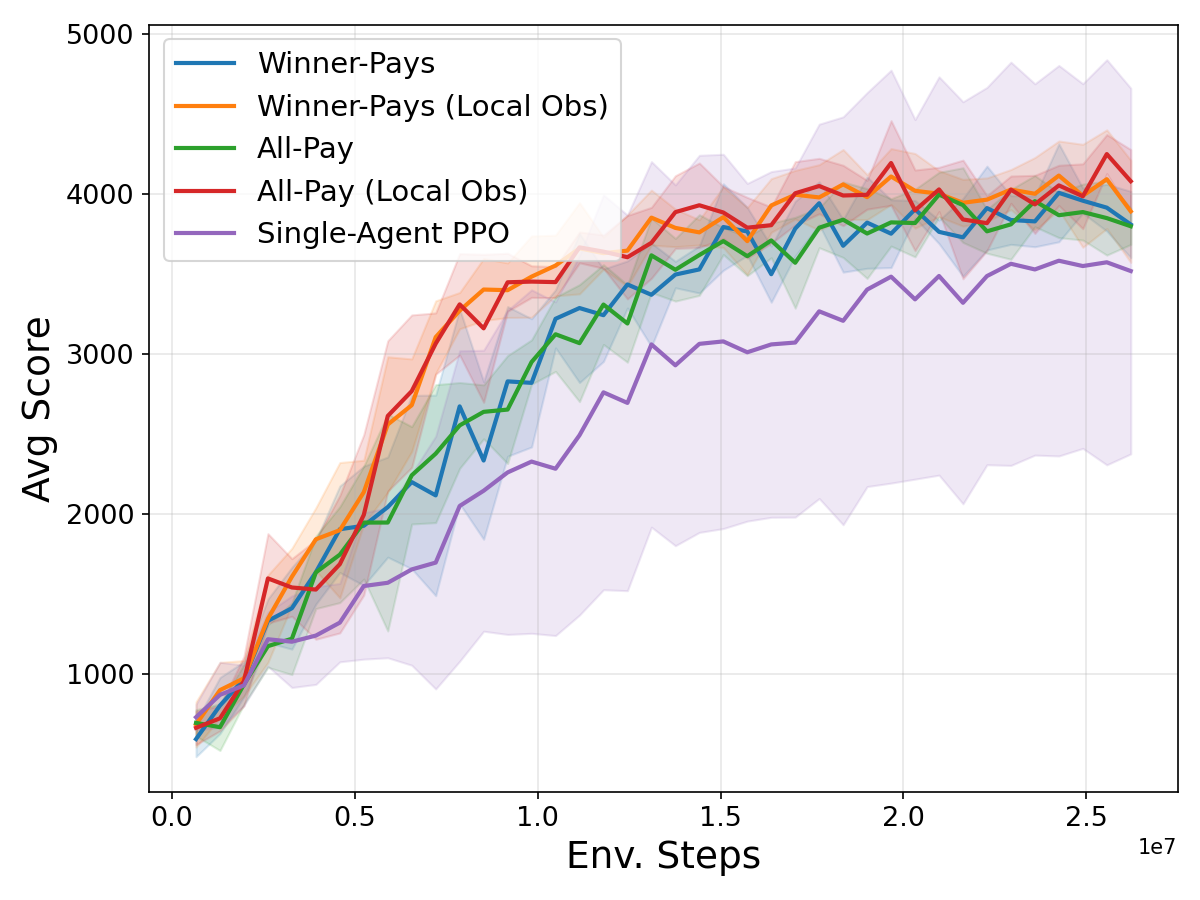
\includegraphics[width=\textwidth]{img/airraid_ppo_bidding_learning_curves_avg_score.png}
        % \caption{Atari Air-Raid: Learning curves}
        % \label{fig:airraid-learning-curves}
    \end{subfigure}
    \caption{Learning curves for different methods on Cat Feeder (left), Atari Assault (center), and Atari Air-Raid (right). We plot mean over 10 seeds at each evaluation iteration and the shaded region is \(\pm\) standard deviation across seeds.}
    \label{fig:learning-curves}
\end{figure}

% \begin{table}
  \centering
  \caption{Gridworld performance (mean $\pm$ std across available seeds) averaged over each seed's last 5 available evaluation iterations. Values are $8 \times \text{avg performance}$ for bidding/single-agent methods, and $8 \times \text{targets reached} - \text{expired}$ for DWN.}
  \begin{tabular}{ll}
    \hline
    {\bf Algorithm} & {\bf Performance} \\
    \hline
    Winner-Pays & $49.44$ {\small\textcolor{gray}{$(\pm 4.19)$}} \\
    Winner-Pays (Local Obs) & $63.76$ {\small\textcolor{gray}{$(\pm 3.85)$}} \\
    Winner-Pays (No Attn. Pool.) & $51.72$ {\small\textcolor{gray}{$(\pm 3.97)$}} \\
    All-Pay & $72.52$ {\small\textcolor{gray}{$(\pm 4.23)$}} \\
    All-Pay (Local Obs) & $64.96$ {\small\textcolor{gray}{$(\pm 3.82)$}} \\
    All-Pay (No Attn. Pool.) & $37.72$ {\small\textcolor{gray}{$(\pm 50.32)$}} \\
    DWN & $-10.27$ {\small\textcolor{gray}{$(\pm 2.38)$}} \\
    Single-Agent PPO & $-51.59$ {\small\textcolor{gray}{$(\pm 5.33)$}} \\
    Single-Agent (NS) & $-14.15$ {\small\textcolor{gray}{$(\pm 41.88)$}} \\
    Single-Agent (ES) & $-47.62$ {\small\textcolor{gray}{$(\pm 1.52)$}} \\
    \hline
  \end{tabular}
  \label{tab:gridworld_methods}
\end{table}

% \begin{table}
  \centering
  \caption{Assault score (mean $\pm$ std across available seeds) averaged over each seed's last 5 evaluation iterations.}
  \begin{tabular}{ll}
    \hline
    {\bf Algorithm} & {\bf Score} \\
    \hline
    Winner-Pays & $556.05$ {\small\textcolor{gray}{$(\pm 29.23)$}} \\
    Winner-Pays (Local Obs) & $557.55$ {\small\textcolor{gray}{$(\pm 36.92)$}} \\
    All-Pay & $576.64$ {\small\textcolor{gray}{$(\pm 43.19)$}} \\
    All-Pay (Local Obs) & $564.36$ {\small\textcolor{gray}{$(\pm 20.68)$}} \\
    DWN & $310.80$ {\small\textcolor{gray}{$(\pm 159.54)$}} \\
    Single-Agent PPO & $358.60$ {\small\textcolor{gray}{$(\pm 25.99)$}} \\
    \hline
  \end{tabular}
  \label{tab:assault_methods}
\end{table}

\begin{table}
  \caption{Scores: mean (standard deviation) across 10 seeds. For all PPO variants, including local observations only, each seed average uses its last 5 available evaluation checkpoints (evaluations every 10 PPO iterations, 20 rollouts each). Cat Feeder score is completed minus expired requests; Atari scores are game scores.}
  \label{tab:all_methods_comp}
  \centering
  \begin{tabular}{llll}
    \toprule
    {\bf Method} & {\bf Cat Feeder} & {\bf Atari Assault} & {\bf Atari Air-raid} \\
    \midrule
    Winner-Pays & $49.44$ {\small\textcolor{gray}{$(4.19)$}} & $556.05$ {\small\textcolor{gray}{$(29.23)$}} & $\textbf{3902.55}$ {\small\textcolor{gray}{$(90.44)$}} \\
    \textcolor{gray}{\itshape\hspace{1em}w. No Attn. Pool.} & \textcolor{gray}{\itshape $51.72$ {\small$(3.97)$}} & \textcolor{gray}{\itshape ---} & \textcolor{gray}{\itshape ---} \\
    \textcolor{gray}{\itshape\hspace{1em}w. Local Obs. Only} & $55.80$ {\small\textcolor{gray}{$(11.42)$}} & --- & --- \\
    All-Pay & $\textbf{72.52}$ {\small\textcolor{gray}{$(4.23)$}} & $\textbf{576.64}$ {\small\textcolor{gray}{$(43.19)$}} & $\textbf{3870.45}$ {\small\textcolor{gray}{$(76.72)$}} \\
    \textcolor{gray}{\itshape\hspace{1em}w. No Attn. Pool.} & \textcolor{gray}{\itshape $37.72$ {\small$(50.32)$}} & \textcolor{gray}{\itshape ---} & \textcolor{gray}{\itshape ---} \\
    \textcolor{gray}{\itshape\hspace{1em}w. Local Obs. Only} & $67.55$ {\small\textcolor{gray}{$(3.79)$}} & --- & --- \\
    \midrule
    DWN & $-10.27$ {\small\textcolor{gray}{$(2.38)$}} & $310.80$ {\small\textcolor{gray}{$(159.54)$}} & $2438.38$ {\small\textcolor{gray}{$(625.97)$}} \\
    Single-Policy PPO & \textcolor{gray}{\itshape ---} & $\textbf{358.60}$ {\small\textcolor{gray}{$(25.99)$}} & $\textbf{3549.33}$ {\small\textcolor{gray}{$(1170.14)$}} \\
    \textcolor{gray}{\itshape\hspace{1em}w. No Reward Shaping} & \textcolor{gray}{\itshape $-51.59$ {\small$(5.33)$}} & \textcolor{gray}{\itshape ---} & \textcolor{gray}{\itshape ---} \\
    \textcolor{gray}{\itshape\hspace{1em}w. Nearest Shaping} & \textcolor{gray}{\itshape $-14.15$ {\small$(41.88)$}} & \textcolor{gray}{\itshape ---} & \textcolor{gray}{\itshape ---} \\
    \textcolor{gray}{\itshape\hspace{1em}w. Expiry Shaping} & \textcolor{gray}{\itshape $-47.62$ {\small$(1.52)$}} & \textcolor{gray}{\itshape ---} & \textcolor{gray}{\itshape ---} \\
    \textcolor{gray}{\itshape\hspace{1em}w. Urgency Weighting} & $51.78$ {\small\textcolor{gray}{$(14.31)$}} & --- & --- \\
    \bottomrule
  \end{tabular}
\end{table}



\textbf{Learning dynamics.}\quad \Cref{fig:learning-curves} shows the learning curves for multi-policy bidding and single-policy PPO algorithms on the three environments.
While the curves are more noisy with Atari Assault, they exhibit clearly distinguishable sigmoidal shapes with the other two environments.
The curves for \allpay and \poorman methods start growing around the same time.
\textbf{The variants without attention pooling for targets only start learning much later.}
This validates the use of the attention pooling architecture to learn useful embeddings of targets.
We remark that, based on the multi-agent PPO recipe of Yu et al.~\citep{yu2022mappo}, we also found that using a small clip coefficient (\({\sim}0.05\)) and large batch sizes was crucial to obtain stable but slower convergence of the policies towards an equilibrium.

\textbf{Comparison with baselines.}\quad \Cref{tab:all_methods_comp} lists performance across the three base environments.
Urgency-weighted scalarization raises centralized PPO's Cat Feeder score to $51.78\pm14.31$, comparable in mean to Winner-Pays ($49.44\pm4.19$), while All-Pay achieves $72.52\pm4.23$.
Thus the stronger baseline changes the comparison materially: All-Pay retains an advantage, whereas Winner-Pays does not outperform urgency-weighted PPO in mean score.
Separating objective rewards may ease credit assignment, but these comparisons do not isolate its causal contribution.
In Assault, single extracted frames may omit velocities and projectile directions; the four-frame observations in Air-Raid may reduce this partial observability.
We did not conduct a dedicated frame-stack ablation, so this remains a possible explanation rather than an established effect.

DWN is included as a closely related multi-policy MORL method that learns a state-dependent arbitration signal.
Its low scores suggest that TD-error-based arbitration is less effective in these experiments; they do not establish that its architecture alone causes the difference.
Our empirical comparisons concern this PPO implementation, rather than a general replacement for PPO across domains.

\textbf{Observations and pooling.}\quad
The non-pooled variants retain all target information through fixed concatenation.
Winner-Pays scores with and without pooling ($49.44\pm4.19$ versus $51.72\pm3.97$) are close relative to the across-seed variation; this does not establish superiority of the non-pooled architecture.
Pooling supports variable-size objective sets and earlier learning in the reported curves.
All-Pay with pooling has a higher mean than its blind variant ($67.55\pm3.79$); blind Winner-Pays has a higher mean ($55.80$) but greater variability ($11.42$), so the observations do not show a consistent final-score benefit for both auction mechanisms.

\textbf{Heterogeneous objectives and priorities.}\quad
We extend Cat Feeder to eight cats with feeding priorities from 1 to 4 and three charging stations, all moving stochastically on a $30\times30$ grid.
The robot has a capacity-50 battery; depletion away from a station triggers a tow and refill.
One local policy serves each cat, and a separate charging policy receives a battery-dependent effective bid boost (Appendix~\ref{app:heterogeneous-implementation}).
Feeding rewards scale with cat priority.
Table~\ref{tab:heterogeneous-cat-feeder} reports the sum of priorities of fed cats and battery depletions, against centralized PPO with an unweighted reward sum.
All-Pay achieves a higher feeding score and fewer battery depletions than centralized PPO, demonstrating coordination across feeding and charging objectives; the nonzero depletion rate does not constitute a safety guarantee.
Appendix~\ref{app:heterogeneous-results} reports feeding counts by priority.

\begin{table}[t]
  \caption{Heterogeneous Cat Feeder: mean (standard deviation) of priority-weighted feeding score and battery depletions. Higher feeding scores and fewer depletions are better.}
  \label{tab:heterogeneous-cat-feeder}
  \centering
  \begin{tabular}{lrr}
    \toprule
    Method & Feeding priority sum & Battery depletions \\
    \midrule
    All-Pay & $194.56\;(4.67)$ & $0.07\;(0.05)$ \\
    Centralized PPO & $111.86\;(57.08)$ & $3.81\;(5.03)$ \\
    \bottomrule
  \end{tabular}
\end{table}


\begin{figure}[h]
    \centering
    \begin{subfigure}[t]{0.31\textwidth}
        \centering
        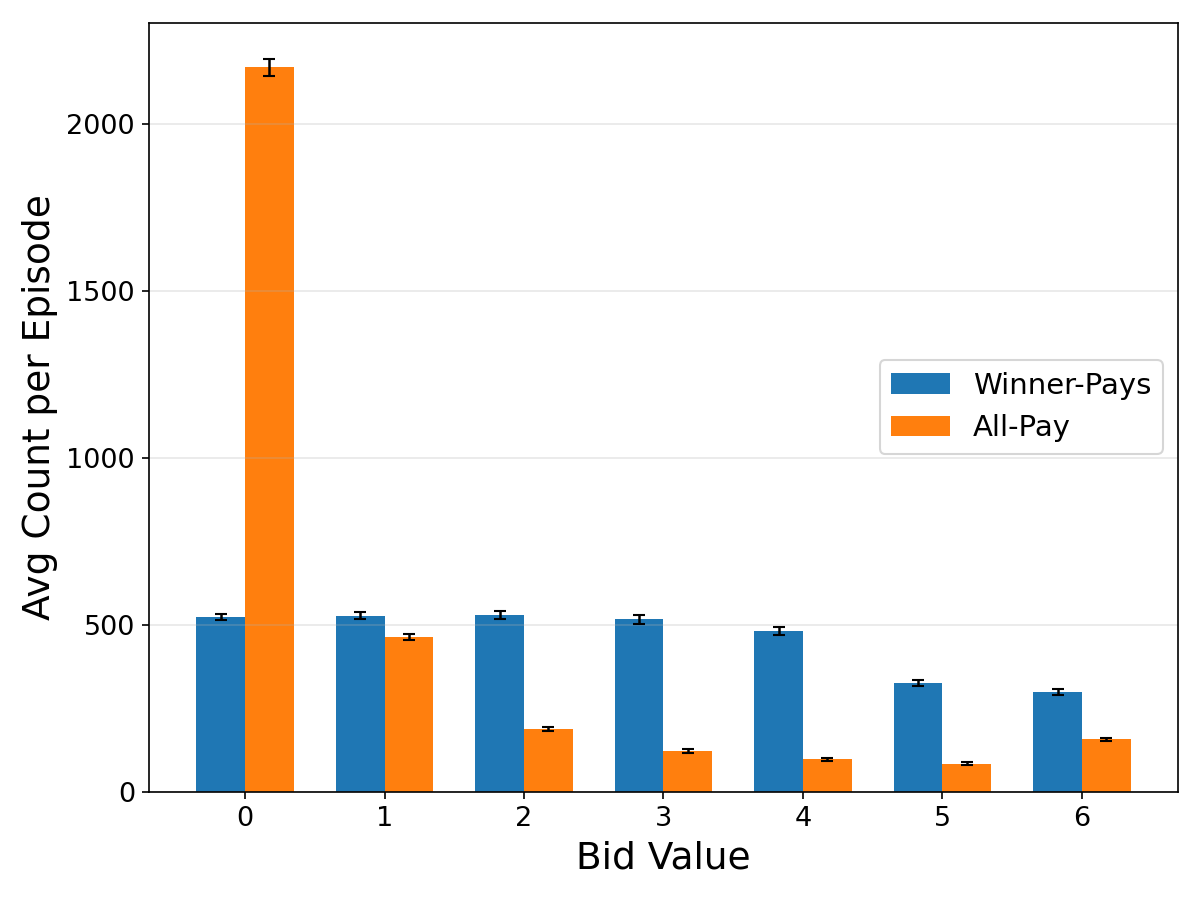
\includegraphics[width=\textwidth]{img/bidding_mechanisms_bid_distribution.png}
        \caption{Cat Feeder: Bid distribution}
        \label{fig:dyntar-bid-dist}
    \end{subfigure}
    \hfill
    \begin{subfigure}[t]{0.25\textwidth}
        \centering
        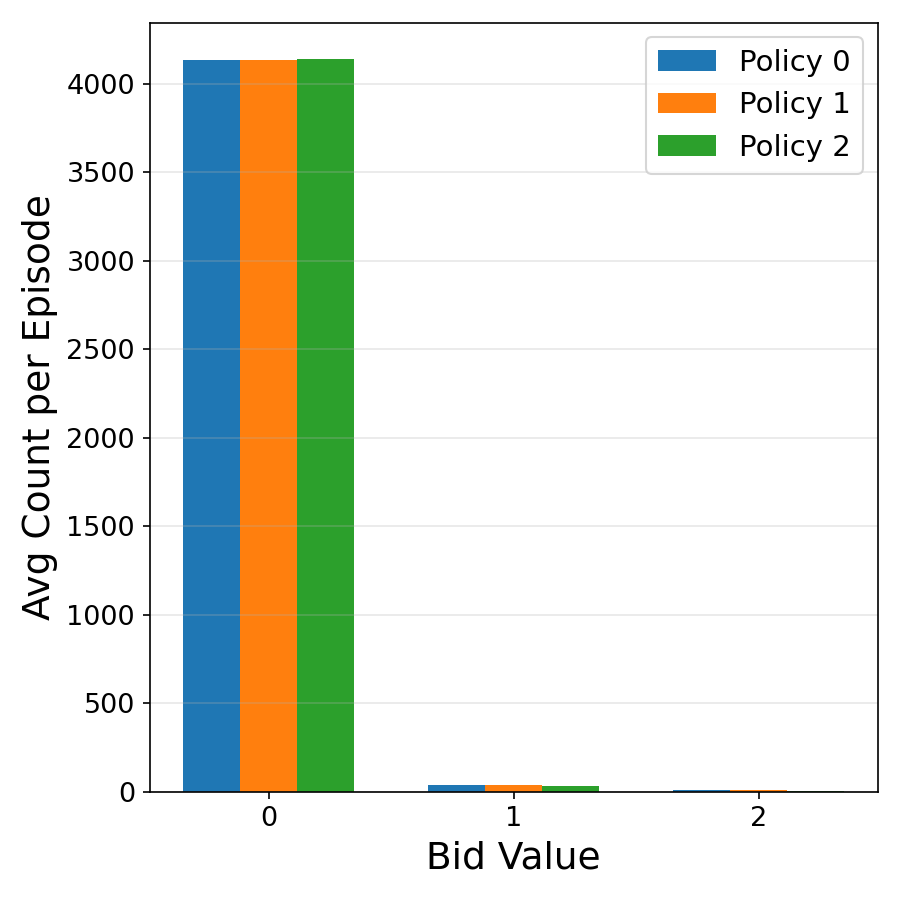
\includegraphics[width=\textwidth]{img/assault_bid_distribution_winner-pays.png}
        \caption{Atari Assault: Bid distribution (\poorman)}
        \label{fig:assault-bid-dist}
    \end{subfigure}
    \hfill
    \begin{subfigure}[t]{0.25\textwidth}
        \centering
        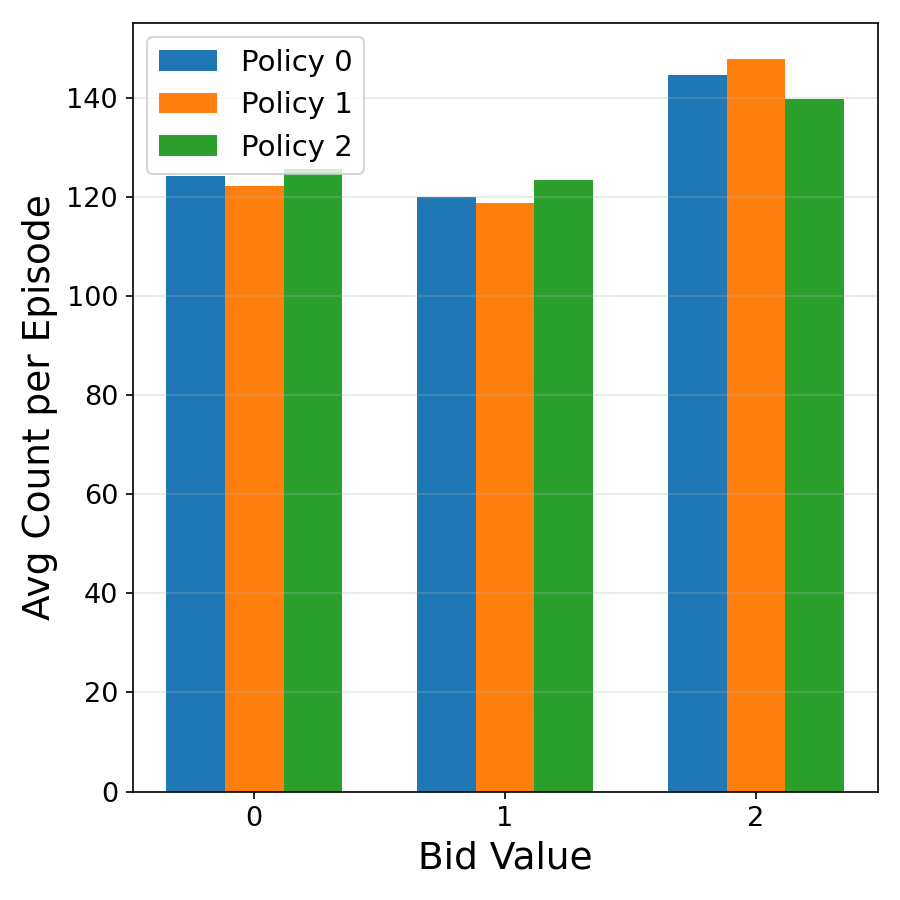
\includegraphics[width=\textwidth]{img/airraid_bid_distribution_winner_pays.png}
        \caption{Atari Air-Raid: Bid distribution (\poorman)}
        \label{fig:airraid-bid-dist}
    \end{subfigure}
    \caption{Comparison of bid distributions across environments and methods. Bars show aggregate bid counts for each bid value across all policies.}
    \label{fig:control-bid-dist}
\end{figure}

\begin{figure}
    \centering
    \begin{subfigure}[b]{0.3\textwidth}
        \centering
        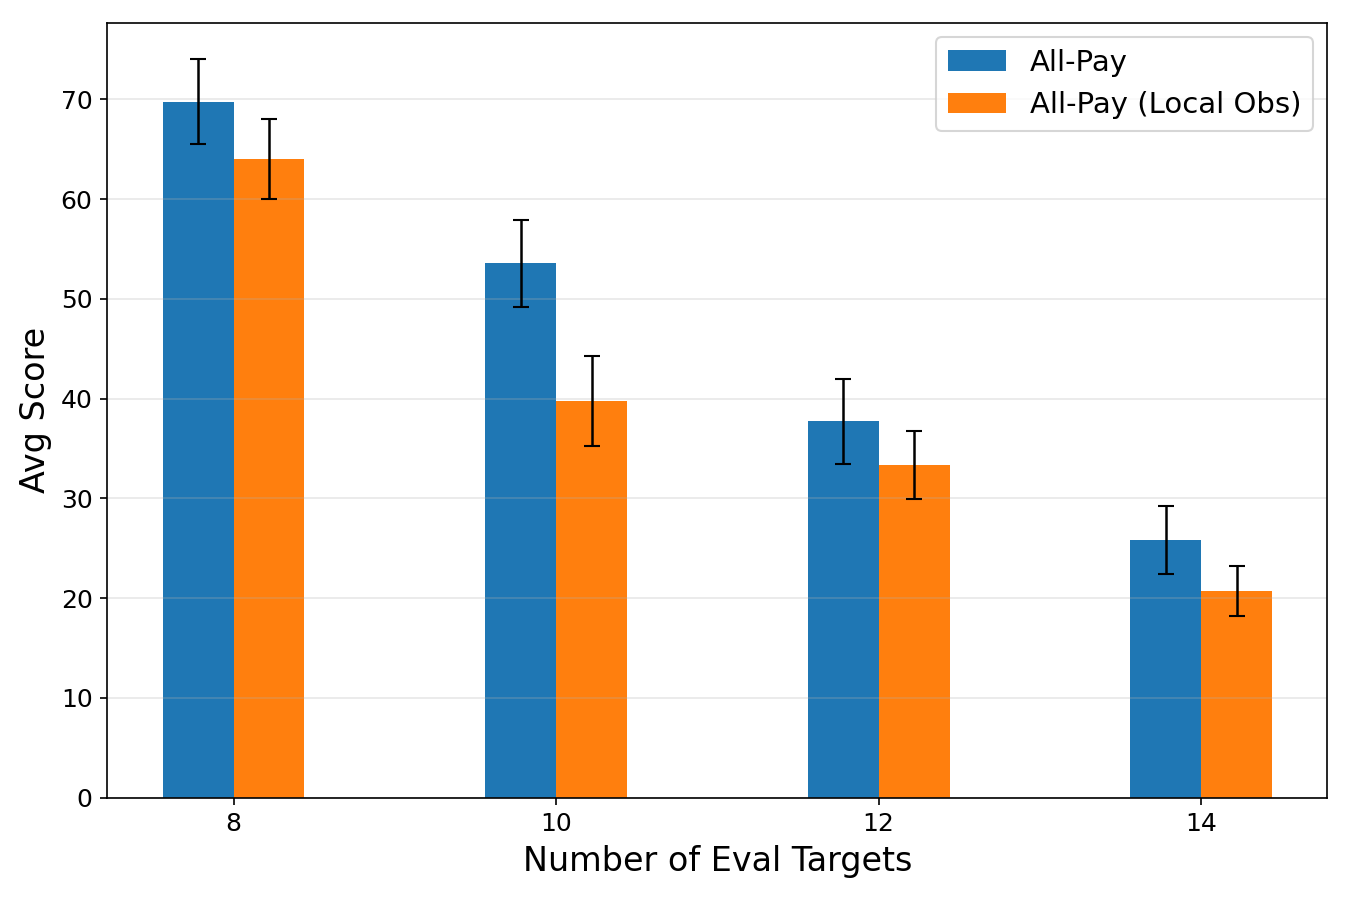
\includegraphics[width=\textwidth]{img/bidding_mechanism_scaling.png}
        \caption{Scaling number of targets.}
        \label{fig:bidding-mechanism-scaling}
    \end{subfigure}
    \hfill
    \begin{subfigure}[b]{0.3\textwidth}
        \centering
        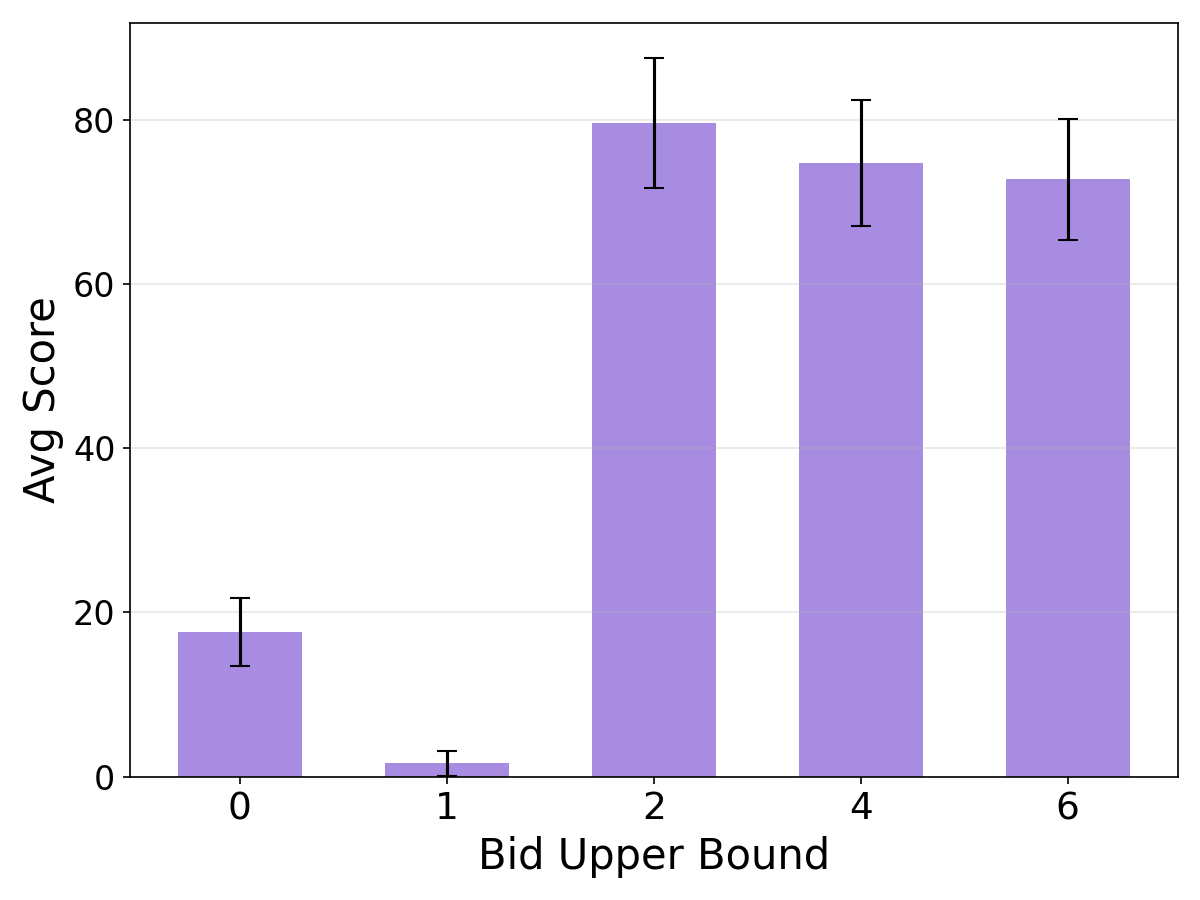
\includegraphics[width=\textwidth]{img/gridworld_bid_upper_bound_bar_chart.png}
        \caption{Ablation: Bid upper bound}
        \label{fig:gridworld-bid-upper-bound}
    \end{subfigure}
    \hfill
    \begin{subfigure}[b]{0.3\textwidth}
        \centering
        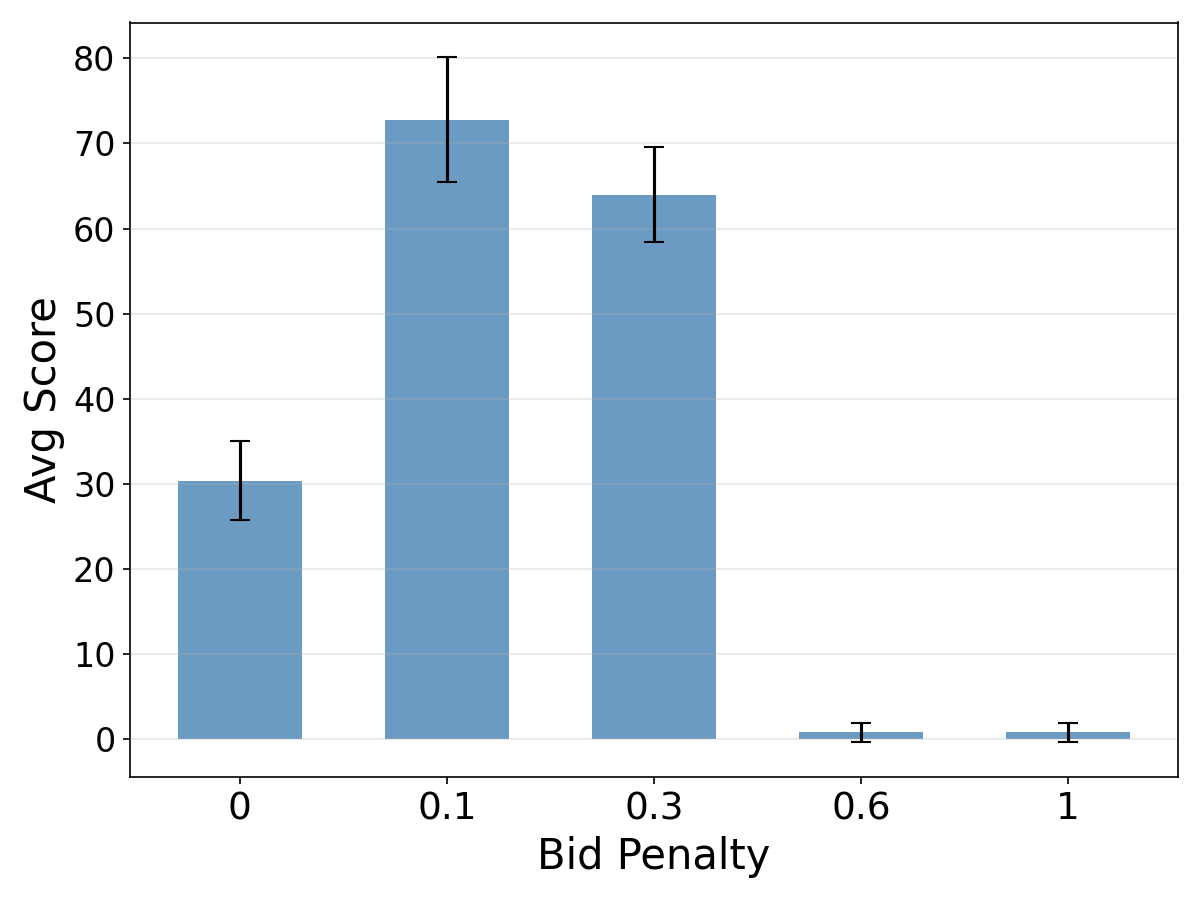
\includegraphics[width=\textwidth]{img/gridworld_bid_penalty_bar_chart.png}
        \caption{Ablation: Bid penalty}
        \label{fig:gridworld-bid-penalty}
    \end{subfigure}
    \caption{Scaling number of targets and ablations on the Cat Feeder environment.}
    \label{fig:ablations}
\end{figure}



\textbf{Policy behaviors and interpretability.}\quad
Video rollouts illustrate control allocation as each policy pursues its assigned objective; completion need not occur within one action window. \Cref{fig:control-bid-dist} presents the bid distributions.
% and control distributions are reported in Appendix~\ref{app:additional-experimental-results}.
In Assault, bids are usually 0, making allocation close to random tie-breaking; the gains here may arise primarily from objective decomposition rather than learned urgency arbitration. In contrast, the Cat Feeder environment shows a wider bid spread (0--6). Here, \allpay yields more conservative policies with mostly low bids, while \poorman produces a more even distribution, reflecting greater willingness to bid high.
Finally, in Air-raid, we see policies bidding the highest value more often, although they also bid lower values.
This is because there is a constant stream of enemy ships that each policy has to destroy and so they want to take control more often to avoid missing out on points.

\textbf{Scaling number of targets.}\quad We conduct an experiment with the Cat Feeder environment in which the number of cats seen during testing is larger than that during training.
This is achieved by deploying more copies of the same policy that optimize the additional objectives.
\Cref{fig:bidding-mechanism-scaling} evaluates transfer from eight training targets to as many as fourteen testing targets without retraining.
The plot uses eight times mean per-episode average performance; scaling selects a single best periodic checkpoint rather than averaging the final five.
With fixed episode length, more requests can expire as target count grows (Appendix~\ref{app:scaling-coverage}).
The minimum reported per-target completion count remains positive at every tested size (Appendix~\ref{app:scaling-coverage}), supporting continued service across all targets rather than constant performance as their number grows.

\textbf{Hyperparameter ablations.}\quad \Cref{fig:gridworld-bid-upper-bound} shows that at least two bid levels are needed for good performance; with only one level, policies cannot compete effectively. \Cref{fig:gridworld-bid-penalty} evaluates the bid penalty factor: without penalties all policies overbid, hurting performance, while overly large penalties discourage bidding. Additional action-window ablations are reported in Appendix~\ref{app:additional-experimental-results}.
